\documentclass{article}
\usepackage{graphicx}
\usepackage{hyperref}
\usepackage{fancyvrb}
\usepackage{vhistory}
\usepackage{float}
\hypersetup{colorlinks,urlcolor=cyan}
\usepackage[margin=1in]{geometry}
\usepackage{listing}
\usepackage{url}

\usepackage{amsmath}
\usepackage{amssymb}
\usepackage{amsthm}
\usepackage{mathtools} %for use of := symbol mostly.
\usepackage{booktabs} % used for making tables

\usepackage[export]{adjustbox} % allows frame around figure

\usepackage[round]{natbib}


\newcommand{\pnote}[1]{{\langle \text{#1} \rangle}}

\begin{document}

\title{\textbf{TrawlExpert: A Tool for Watershed Biological Research}}
\author{Trawlstars Inc. (Group 11) \\ Lab section: L01  \\ Version: 1.0 \\ SFWRENG 2XB3 \\ \\ Christopher W. Schankula, 400026650, schankuc \\ Haley Glavina, 001412343, glavinhc \\ Winnie Liang, 400074498, liangw15 \\ Ray Liu, 400055250, liuc40 \\ Lawrence Chung, 400014482, chungl1}


\maketitle

\begin{center}

\includegraphics{logo.png}
\end{center}

\newpage

\begin{versionhistory}
  \vhEntry{1.0}{05.04.18}{HG}{created}
  \vhEntry{1.1}{08.04.18}{HG}{algorithmic analysis added}
  \vhEntry{1.2}{10.04.18}{RL}{Added Modular structure and uses}
\end{versionhistory} 

\noindent\textit{By virtue of submitting this document we electronically sign and date that the work being submitted by all the individuals in the group is their exclusive work as a group and we consent to make available the application being developed through SE-2XB3 project, the reports, presentations, and assignments (not including my name and student number) for future teaching purposes.}

\newpage

\textbf{\Large{Team Contributions}}\\ \\
The individual contributions of each team member are described below. Subteam B indicates an algorithmic focus in a member's efforts while Subteam A indicates a focus on data parsing and user interface development. Although the contributions have been separated such that each task is recorded under one contributor, members often overlapped duties and designed modules together. \\

\begin{table}[h]
	\centering
	\begin{tabular}{p{0.16\hsize}p{0.30\hsize}p{0.46\hsize}}
		\toprule
		\textbf{Name} & \textbf{Role} & \textbf{Contributions}\\
		\midrule
		Lawrence Chung
		& Head of Room Booking \newline Subteam B Member
		& Implemented the depth first search and connected components algorithms. \\
		\midrule
		Haley Glavina
		& Meeting Minutes Administrator \newline Subteam B Member
		& Implemented the red-black tree, quickselect, and mergesort algorithms. Designed the final presentation powerpoint, recorded and submitted all meeting minutes, and assembled the final design specification in LaTeX. Generated UML state machine diagrams.\\
		\midrule
		Winnie Liang
		& Project Log Administrator \newline Subteam A Member
		& Implemented the module responsible for parsing out data to create related objects, implemented taxonNode ADT. Led user interface development, set up tomcat files and directory structure,  handled communication between the Google Maps APIs and JavaScript code. Overlooked project log entries.\\
		\midrule
		Ray Liu
		& TA \& Professor Liaison \newline Subteam A Member
		& Implemented Record ADT, Date ADT, parsing API calls for WORMS API, RangeHelper for Basic Search, Histogram output for command line, histogram output for web interface.\\
		\midrule
		Christopher Schankula
		& Team Leader \newline Subteam A Member
		& Determined the goals for each meeting, implemented the k-d tree algorithm, wrote backend of server, wrote command-line tool. \\		
		\bottomrule
	\end{tabular}
\end{table}


\newpage

\begin{abstract}
\noindent \textit{TrawlExpert} is a powerful tool to enable researchers to analyze and filter large datasets from fish trawl surveys in order to perform environmental research on fish and invertebrate populations. The tool gives researchers the ability to intelligently filter and query datasets based on biological classification such as family, genus or species, or based on location or timeframe. Advanced outputs display data as a histogram or geographical map, each depending on population abundance as a function of time and spatial distribution. Additionally, \textit{TrawlExpert} provides a tool for finding local subpopulations within a larger query. A dataset of thousands of Great Lakes trawl surveys from 1958-2016 will be used as a demonstration of \textit{TrawlExpert}'s capability to help researchers narrow down large datasets and glean data which pertains to their research. \textit{TrawlExpert} will be designed to be used easily and effectively as the first step in a groundbreaking climate and ecological research pipeline.
\end{abstract}


\tableofcontents


\section{Project Scope}
\subsection{Objective}
Provide a statistical and visual tool for the analysis of water ecosystems, based on scientific water trawl data. Gives researchers with tools to analyze large datasets to find patterns in fish populations, including the plotting of historical population data on a map, the analysis of population trends over time and the determination of subpopulations of a certain biological classification.

\subsection{Motivation}
The diminishing of fish populations in the Great Lakes became a problem in the latter half of the 20th century, with the total prey fish biomass declining in Lakes Superior, Michigan, Huron and Ontario between 1978 and 2015 \citep{michigan2017}. Annual bottom trawl surveys involve using specialized equipment to sweep an area and are used to determine the relative temporal variation in stock size, mortality and birth rates of different fish species \citep{walsh1997efficiency}. These surveys are performed annually and often have hundreds of thousands of records, making manual analysis infeasible. The ongoing protection and development of the Great Lakes water basins is considered an important topic for scientists in both Canada and the United States, as evidenced by grants such as the \textit{Michigan Sea Grant} \citep{michseagr2018}.

TrawlExpert will give researchers tools to filter through these large amounts of data by allowing them to search through data based on class, order, genus, family or species. This will help support scientific researchers and fishing companies as they study fish populations. These studies help inform initiatives to preserve fish populations and conduct their business in an environmentally friendly way going forward. As more data is collected on an annual basis, TrawlExpert can easily be injected with the new data and will adjust and scale accordingly, combining the new data with the old data for continued analysis.

TrawlExpert will also analyze the trawl data to find connected subpopulations within the data, giving researchers tools to analyze the portions of the water body that contain different populations and even track these specific subpopulations over time.

The focus of the project will be to develop these unique data searching and querying tools as a first step in a complete trawl survey analysis. For a complete analysis, tools like stratified statistical analysis are required by the researcher \citep{walsh1997efficiency}. For purposes of maintaining a manageable scope for this project, the implementation of advanced trawl survey scientific and statistical analysis tools will be relegated to future developments. 

\subsection{Dataset}\label{sec:out}
The test dataset that will be used for purposes of this project is the \textit{USGS Great Lakes Science Center Research Vessel Catch Information System Trawl} published by the United States Geological Survey \citep{usgs2018}. Compiled on yearly operations taking place from early spring to late fall from 1958 until 2016, the dataset contains over 283,000 trawl survey records in the five Great Lakes, including the latitude and longitude co-ordinates and biological classification such as family, genus and species.

\subsection{Final Product}
\begin{figure}
\centering
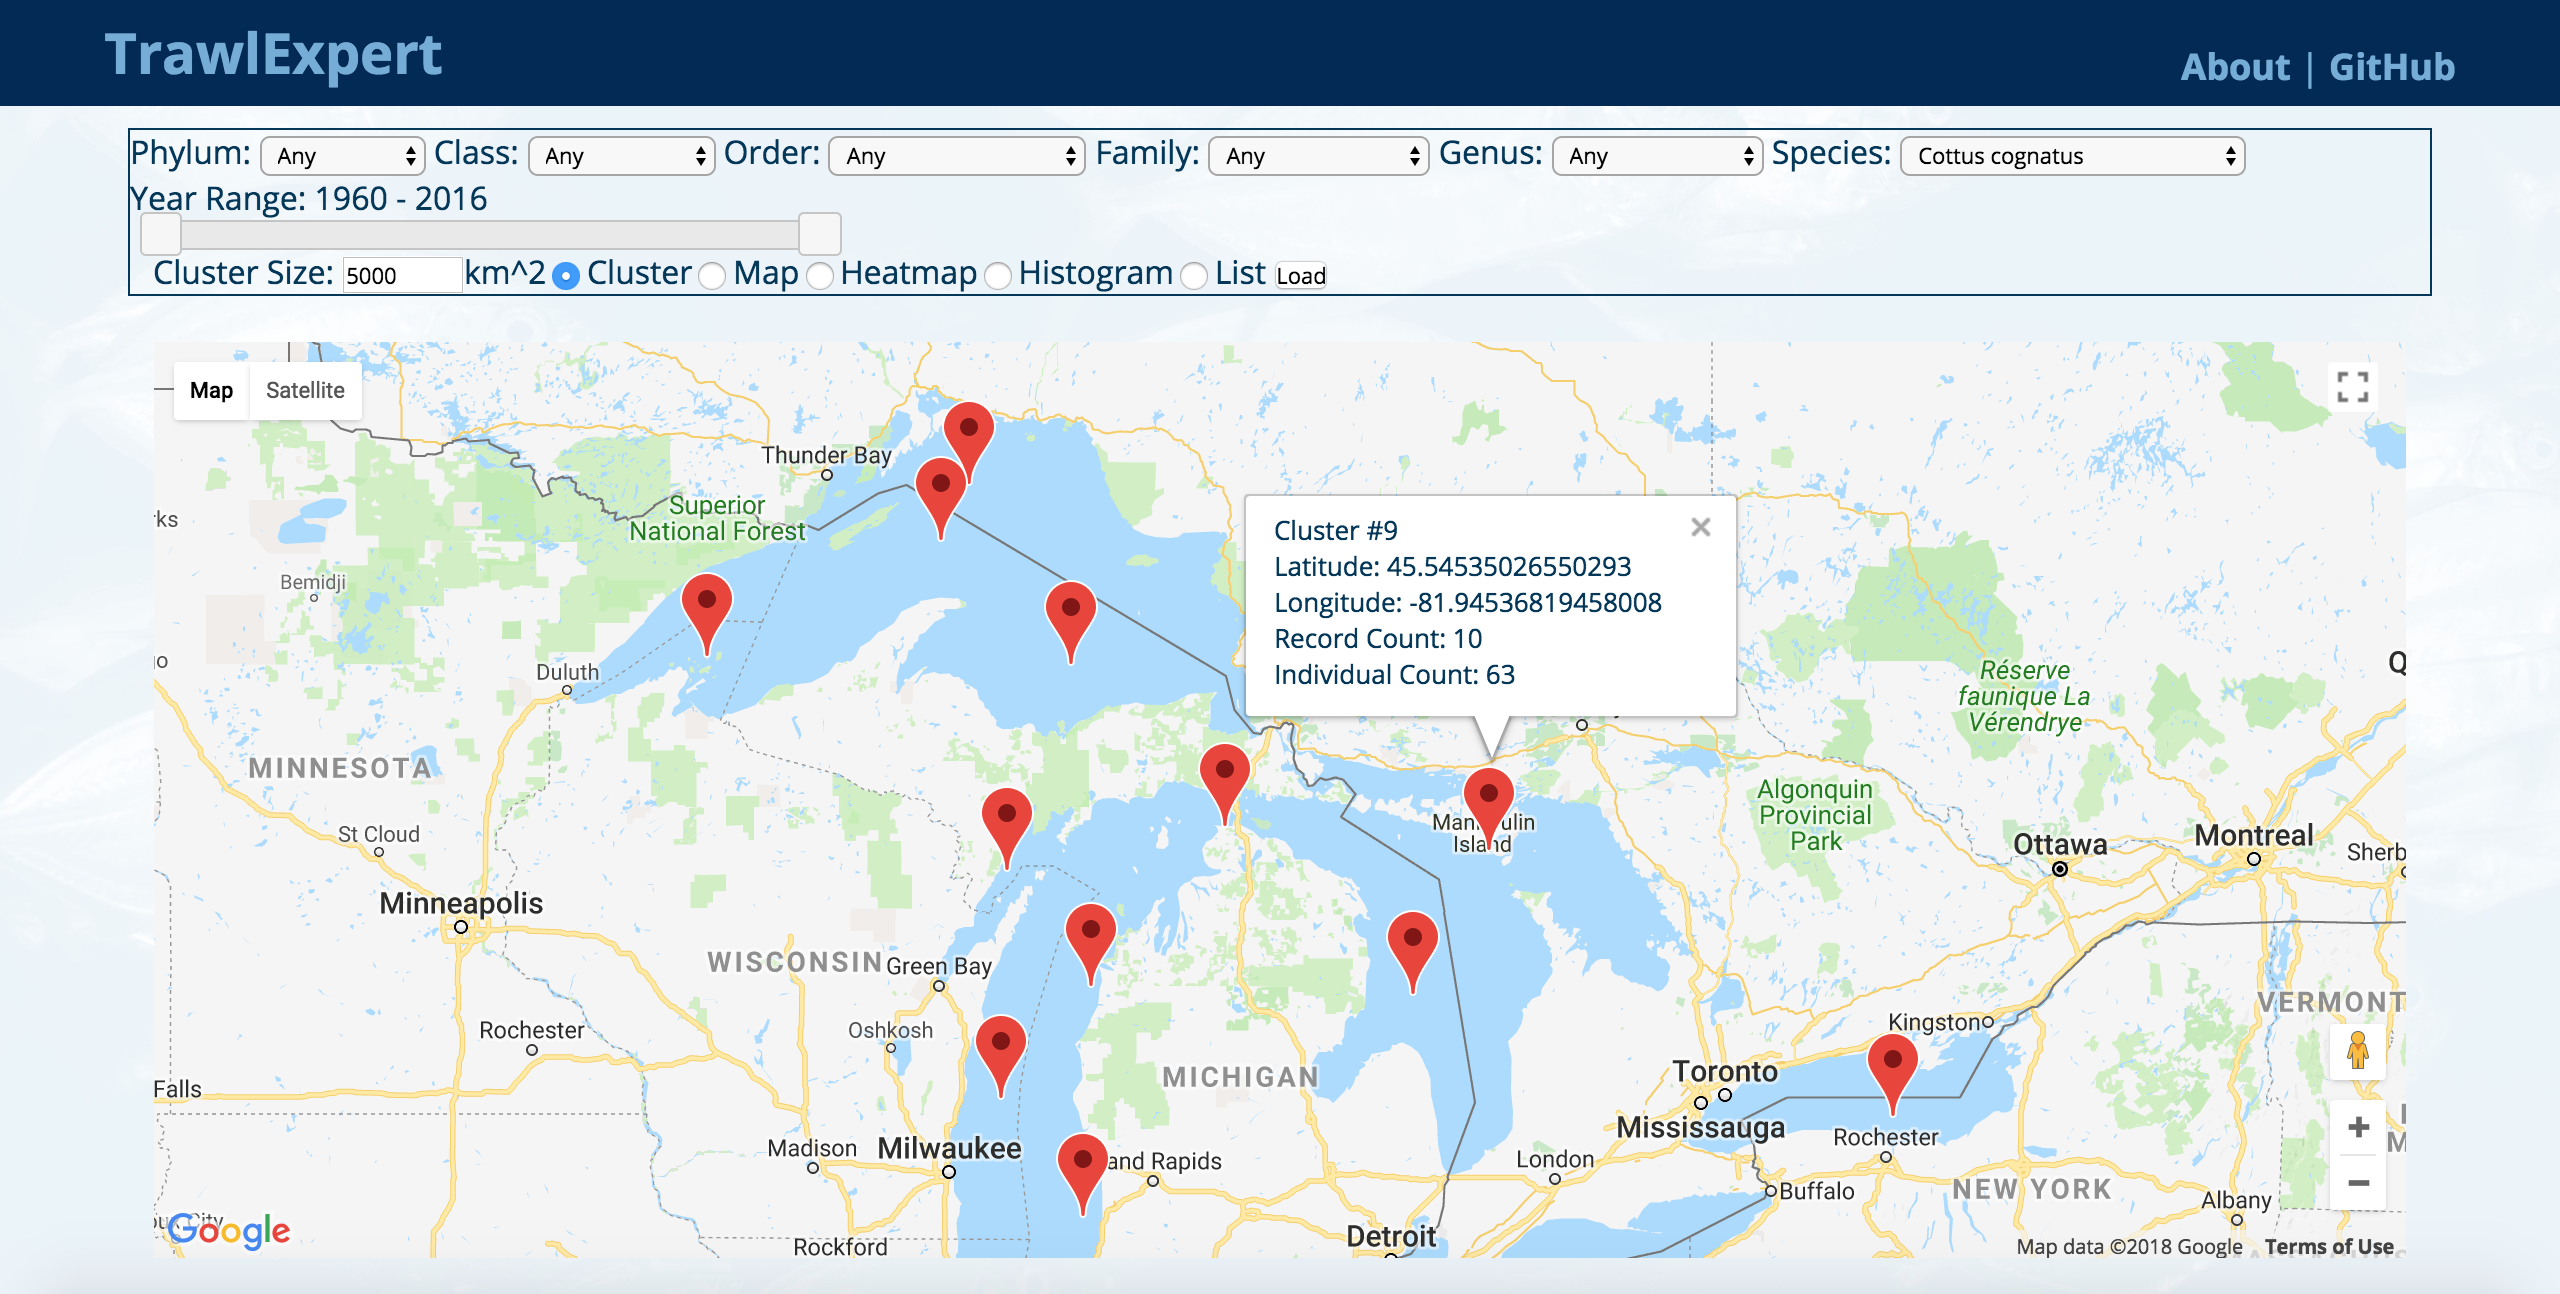
\includegraphics[width=16cm]{UI.png}
\caption{The final TrawlExpert web interface allows users to intelligently search for specific taxa and display several helpful statistical and data visualization tools such as maps and histograms.}
\label{fig:UI}
\end{figure}

Apache tomcat was used to create a webserver which uses the internal functionality and model of TrawlExpert written in Java. The UI allows users to filter by using information about different taxa (their biological relationships to each other, such as family / genus / species, etc) and display several different data outputs such as histograms, heatmaps, maps and population clusters, in addition to viewing raw data in tabular form. The clustering function is shown in \ref{fig:UI}. The \textit{TrawlExpert} is hosted on Google Cloud Platform and can be accessed at \url{http://trawl.schankula.ca/Trawl}. 


\section{Implementation}
\subsection{Classes and Modules}
The implementation involved over 30 classes implemented in Java. Additional JavaScript and HTML files were used to create a sophisticated web-based user interface. For a description of each class and module used, JavaDoc documentation can be viewed by opening the \texttt{doc/index.html} folder in the submission archive or by visiting \url{http://trawl.schankula.ca/Trawl/doc}.


\subsection {Modular Structure and Uses}
The requirements in the Requirement Specification Document are achieved by applying modularity and seperation of concerns, which will be shown in the UML diagrams. The table below traces back to requirements for each class interface:\\

\begin{tabular}{| l | l |}
\hline
\textbf{Requirements} & \textbf{Modules}\\
\hline
Reading input file and dealing with corrupted data (Funcitonal)& WORM.java,FileProcessor.java \\
\hline
List of species by family, order, genus  (Funcitonal)& KDT.java, RangeHelper.java, Quickselect.java \\
\hline
Historical distribution of records  (Funcitonal) & Histogram.java, RedBlackTree.Java, BasicSearch.java \\
\hline
Geographical subgroupings  (Funcitonal) & Graph.java, CC.java \\
\hline
Plotting/mapping tools &  BasicSearch.java, CC.java (With Google Maps API) \\
\hline
Fast Speed (Non-functional) & KDT.java, Quickselect.java, and RedBlackTree.java \\
\hline
Low Memory Usage (Non-functional) & KDT.java, Quickselect.java, and RedBlackTree.java \\
\hline
Scalable (Non-functional) & KDT.java, Quickselect.java, and RedBlackTree.java \\
\hline
\end{tabular}.

\subsection{Class Organization}
An overview of the modules included in the \textit{TrawlExpert} is shown in figure \ref{fig:UML}. The \textit{Trawl Expert} implementation efforts were divided into two subteams: Subteam A and Subteam B. Tasks were assigned so as to maximize the parallelization of the development process. As a biproduct, modules were designed to uphold the principles of information hiding, modularity and separation of concerns.

\subsubsection{model Package}
This class represents the model of the \textit{TrawlExpert} platform. It provides wrapper hooks to functionality deeper inside the codebase, which allows different views to be used separately from the internal functionality. Two such views are the command-line interface in \texttt{main/Main.java} and the tomcat server. This design allows any such view to be built upon the foundation of the model, without needing to edit any underlying code.

\subsubsection{data Package}

\subsubsection{search Package}

\subsubsection{sort Package}

\subsubsection{graph Package}

\subsubsection{utils Package}

\subsubsection{web Package}

\begin{figure}
\centering
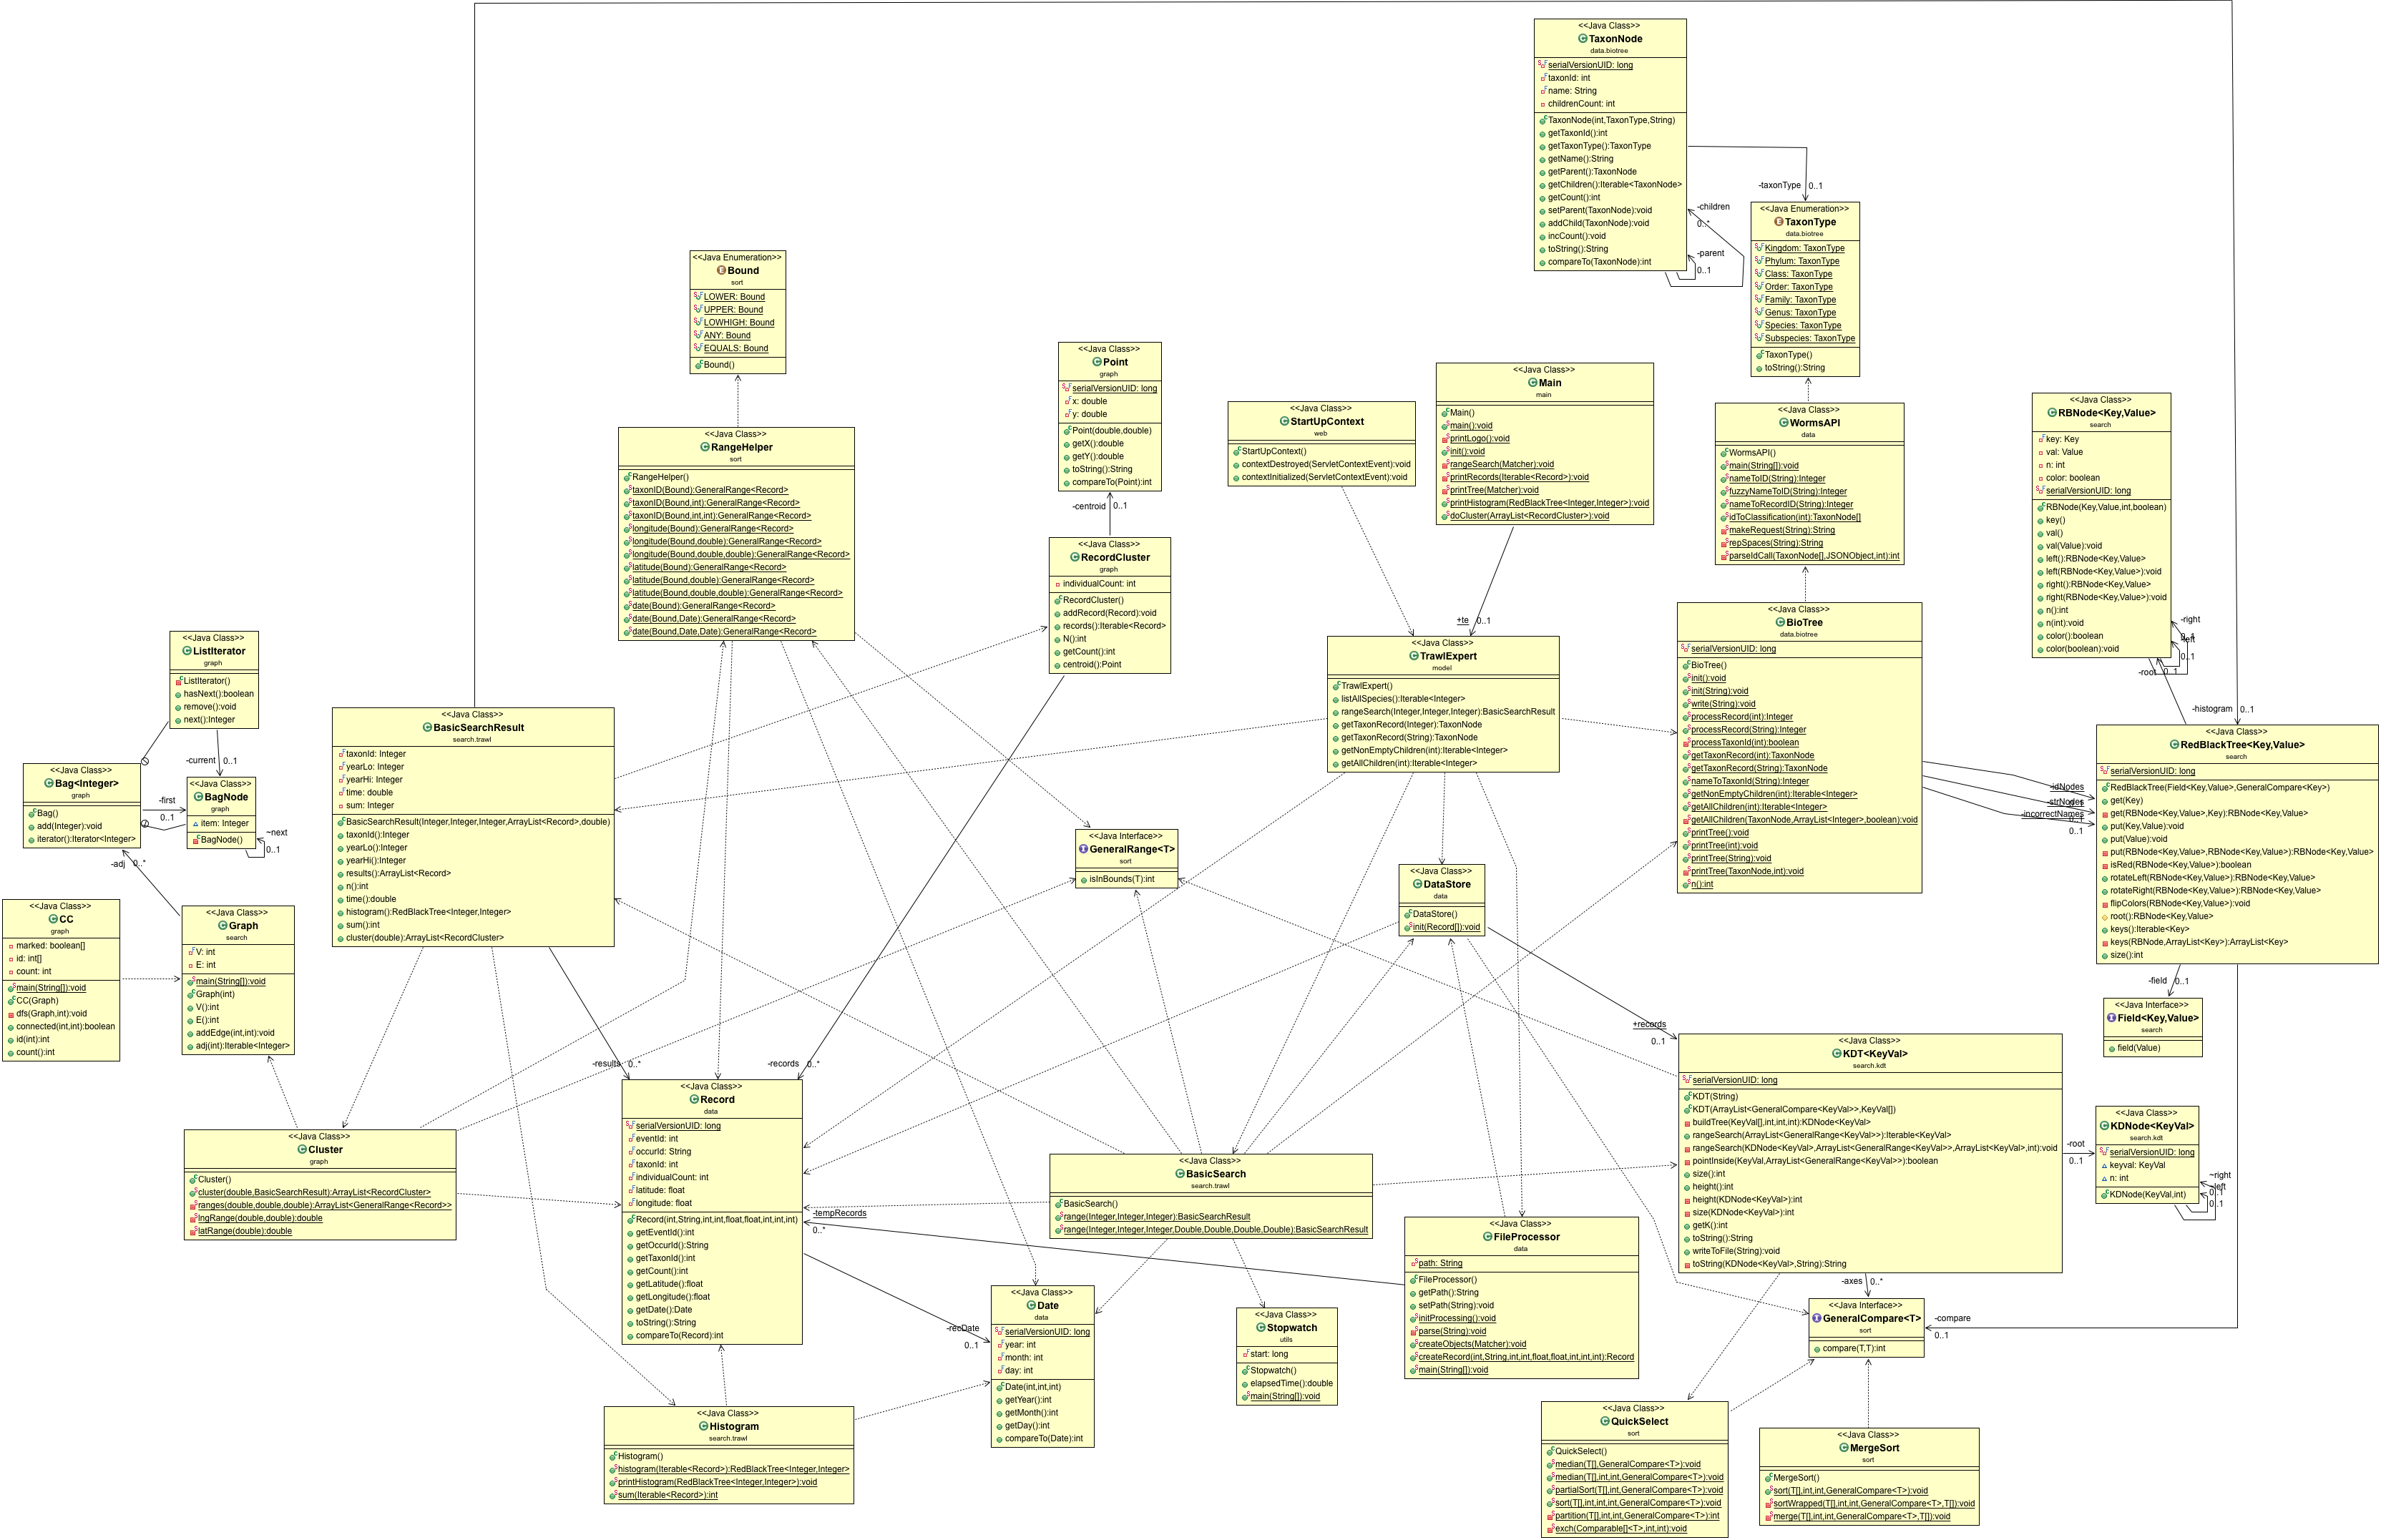
\includegraphics[angle=90,width=14cm]{ClassUML.png}
\caption{The UML class diagram of TrawlExpert, showing the relationships amongst modules. The full-resolution version is available in the root directory of the submission archive as \texttt{UML.png}.}
\label{fig:UML}
\end{figure}


\subsection{UML State Diagrams}
Two UML state machine diagrams are included to describe the states and transitions within the \textit{BioTree.java} and \textit{Main.java} class.

\subsubsection{Main.java}
The UML digrama for the Main.java class is shown in \ref{fig:MainUML}. This represents the \textit{TrawlExpert} console application's states, giving an overview of the types of queries and functions the user has access to. Since the \textit{Main.java} class is a console version of the final server implementation, the states shown in its UML state machine diagram are analogous to many of the states of the final \textit{TrawlExpert} website.
 
\subsubsection{BioTree.java}
The UML state diagram for the BioTree module is shown in figure \ref{fig:BioTreeUML}. The BioTree class is a singleton class which stores the information about the different taxa in the dataset. This method has a few advantages. Firstly, the string names and relationships amongst taxa (e.g. species, genus, family) are stored only once and accessed when needed, saving large amounts of memory compared to the original dataset. For example, the original .csv file of the dataset was approximately 130mb. After running through the TrawlExpert, the serialized dataset representing the same data is only 27mb. This is because there was a large amount of duplication of names on each line of the dataset.

Secondly, this diagrams represents a key feature of \textit{TrawlExpert} in that it is able to recover corrupted data as the dataset is processed, which is very helpful for large datasets. In the USGS dataset, for example, there were 115 instances of different incorrectly named taxa, totalling 15,596 records (almost 6\% of the records in the dataset). Using this method, these records were able to be recovered for proper use by the scientist. Using smart caching of incorrect names described by this UML diagram, the number of API calls to WORMS is kept at a minimum and the dataset processing only takes about 3 minutes. After the initial processing, the BioTree and records are stored as serialized Java objects to the disc, and can be reloaded in less than 10 seconds.

% Include explanations of why we divided it into some of its main sections/classes

\begin{figure}[H]
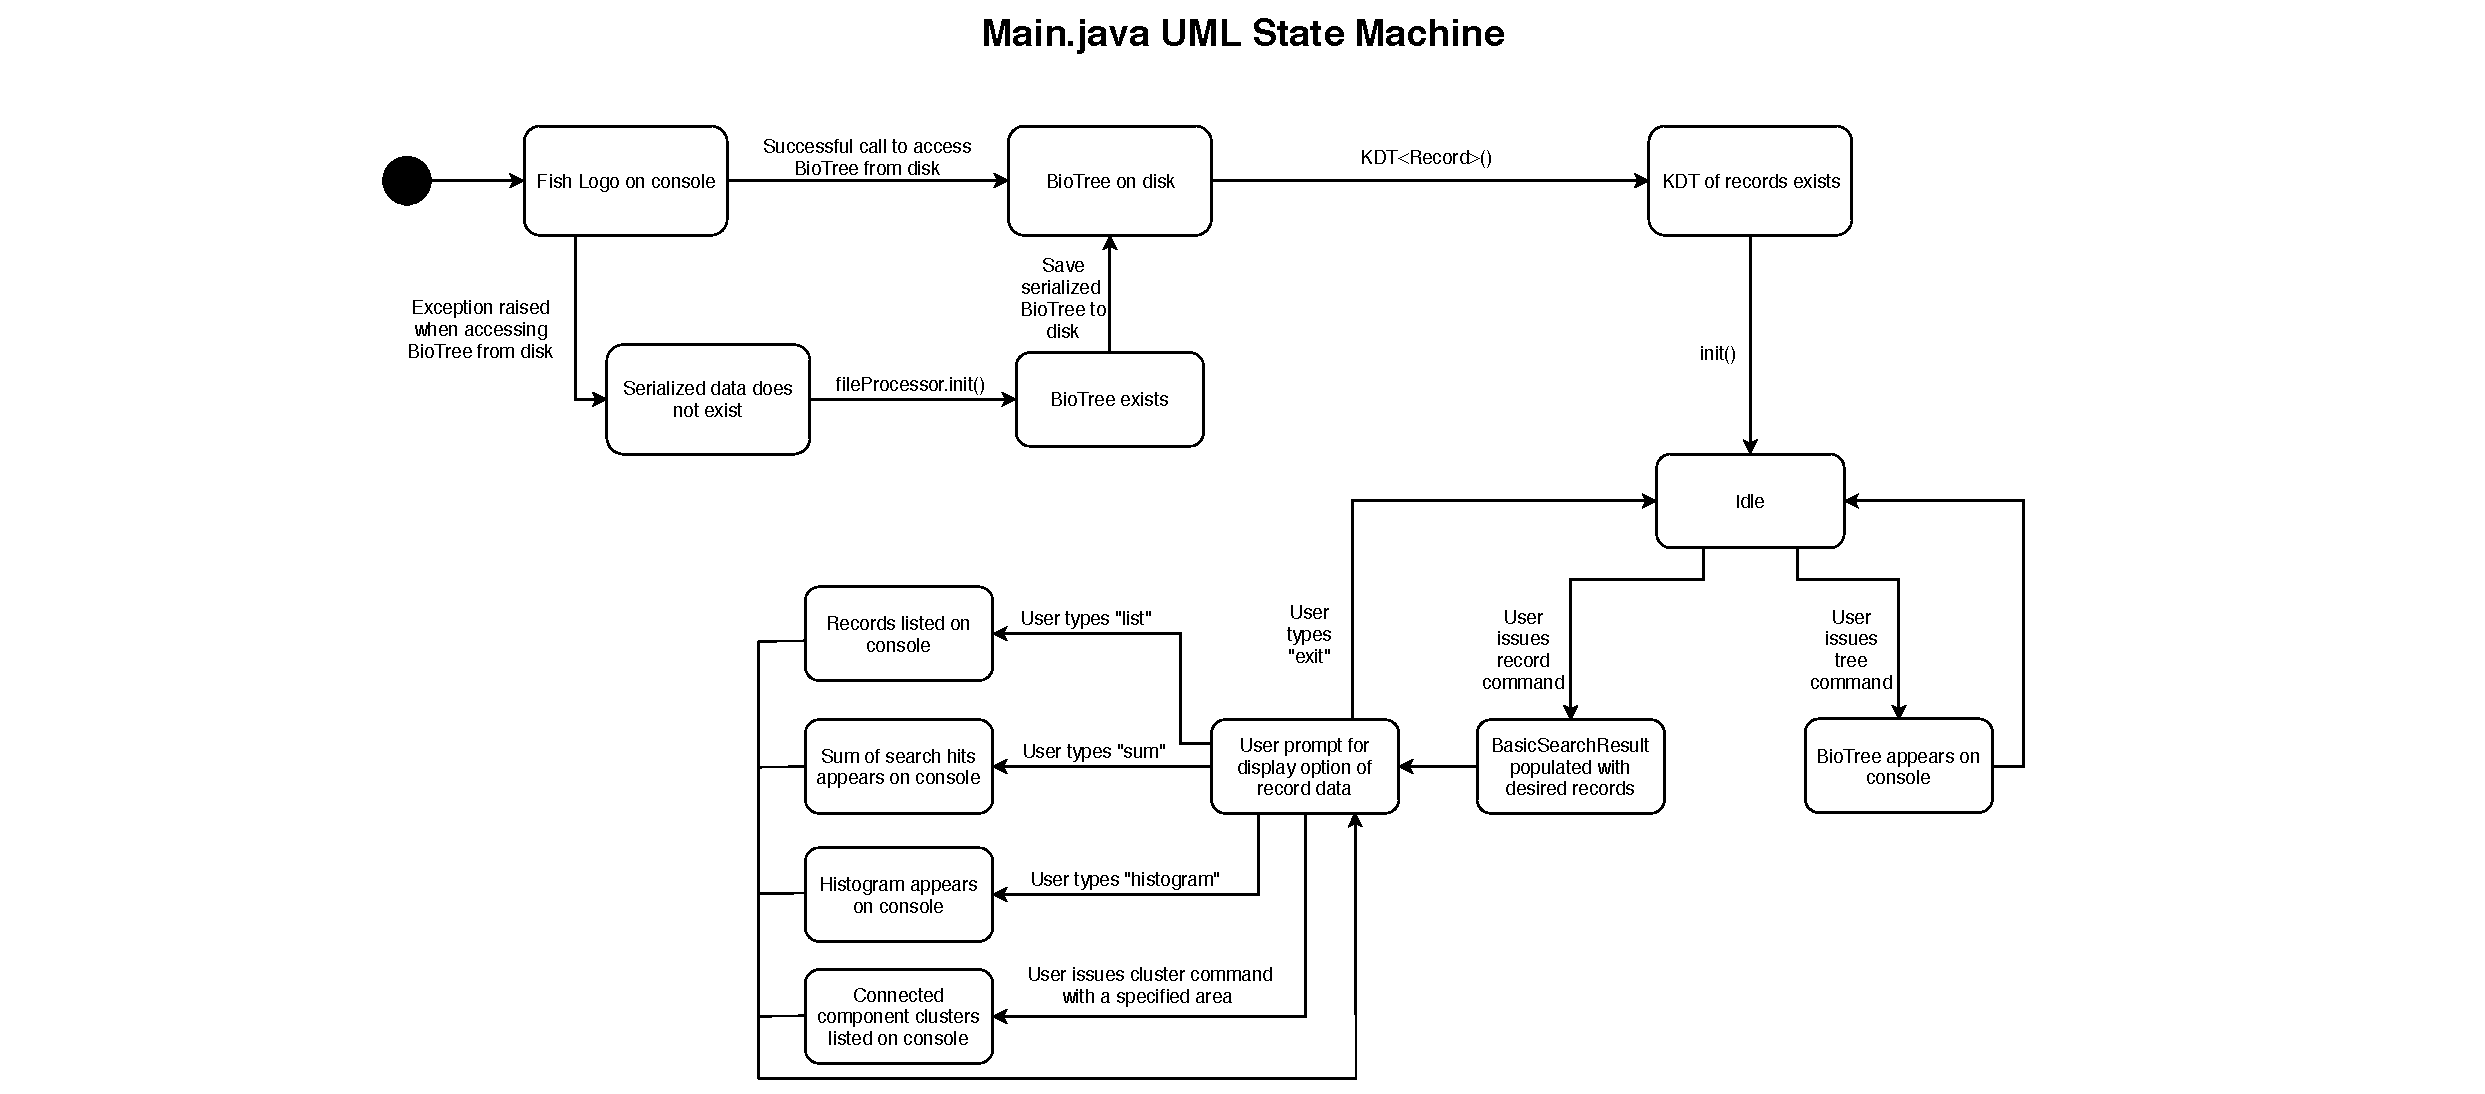
\includegraphics[width=18cm, trim={6cm 0 6cm 0}, clip]{MainDotJava.pdf}

\caption{UML State machine diagram for \textit{main/Main.java}, a class that provides console access to the \textit{TrawlExpert}'s main functions. This class accepts search criteria from a user to produce a list of search results, depict a histogram of the records in that result, and compute a count of the search hits.}
\label{fig:MainUML}
\end{figure}

\begin{figure}[H]
\centering
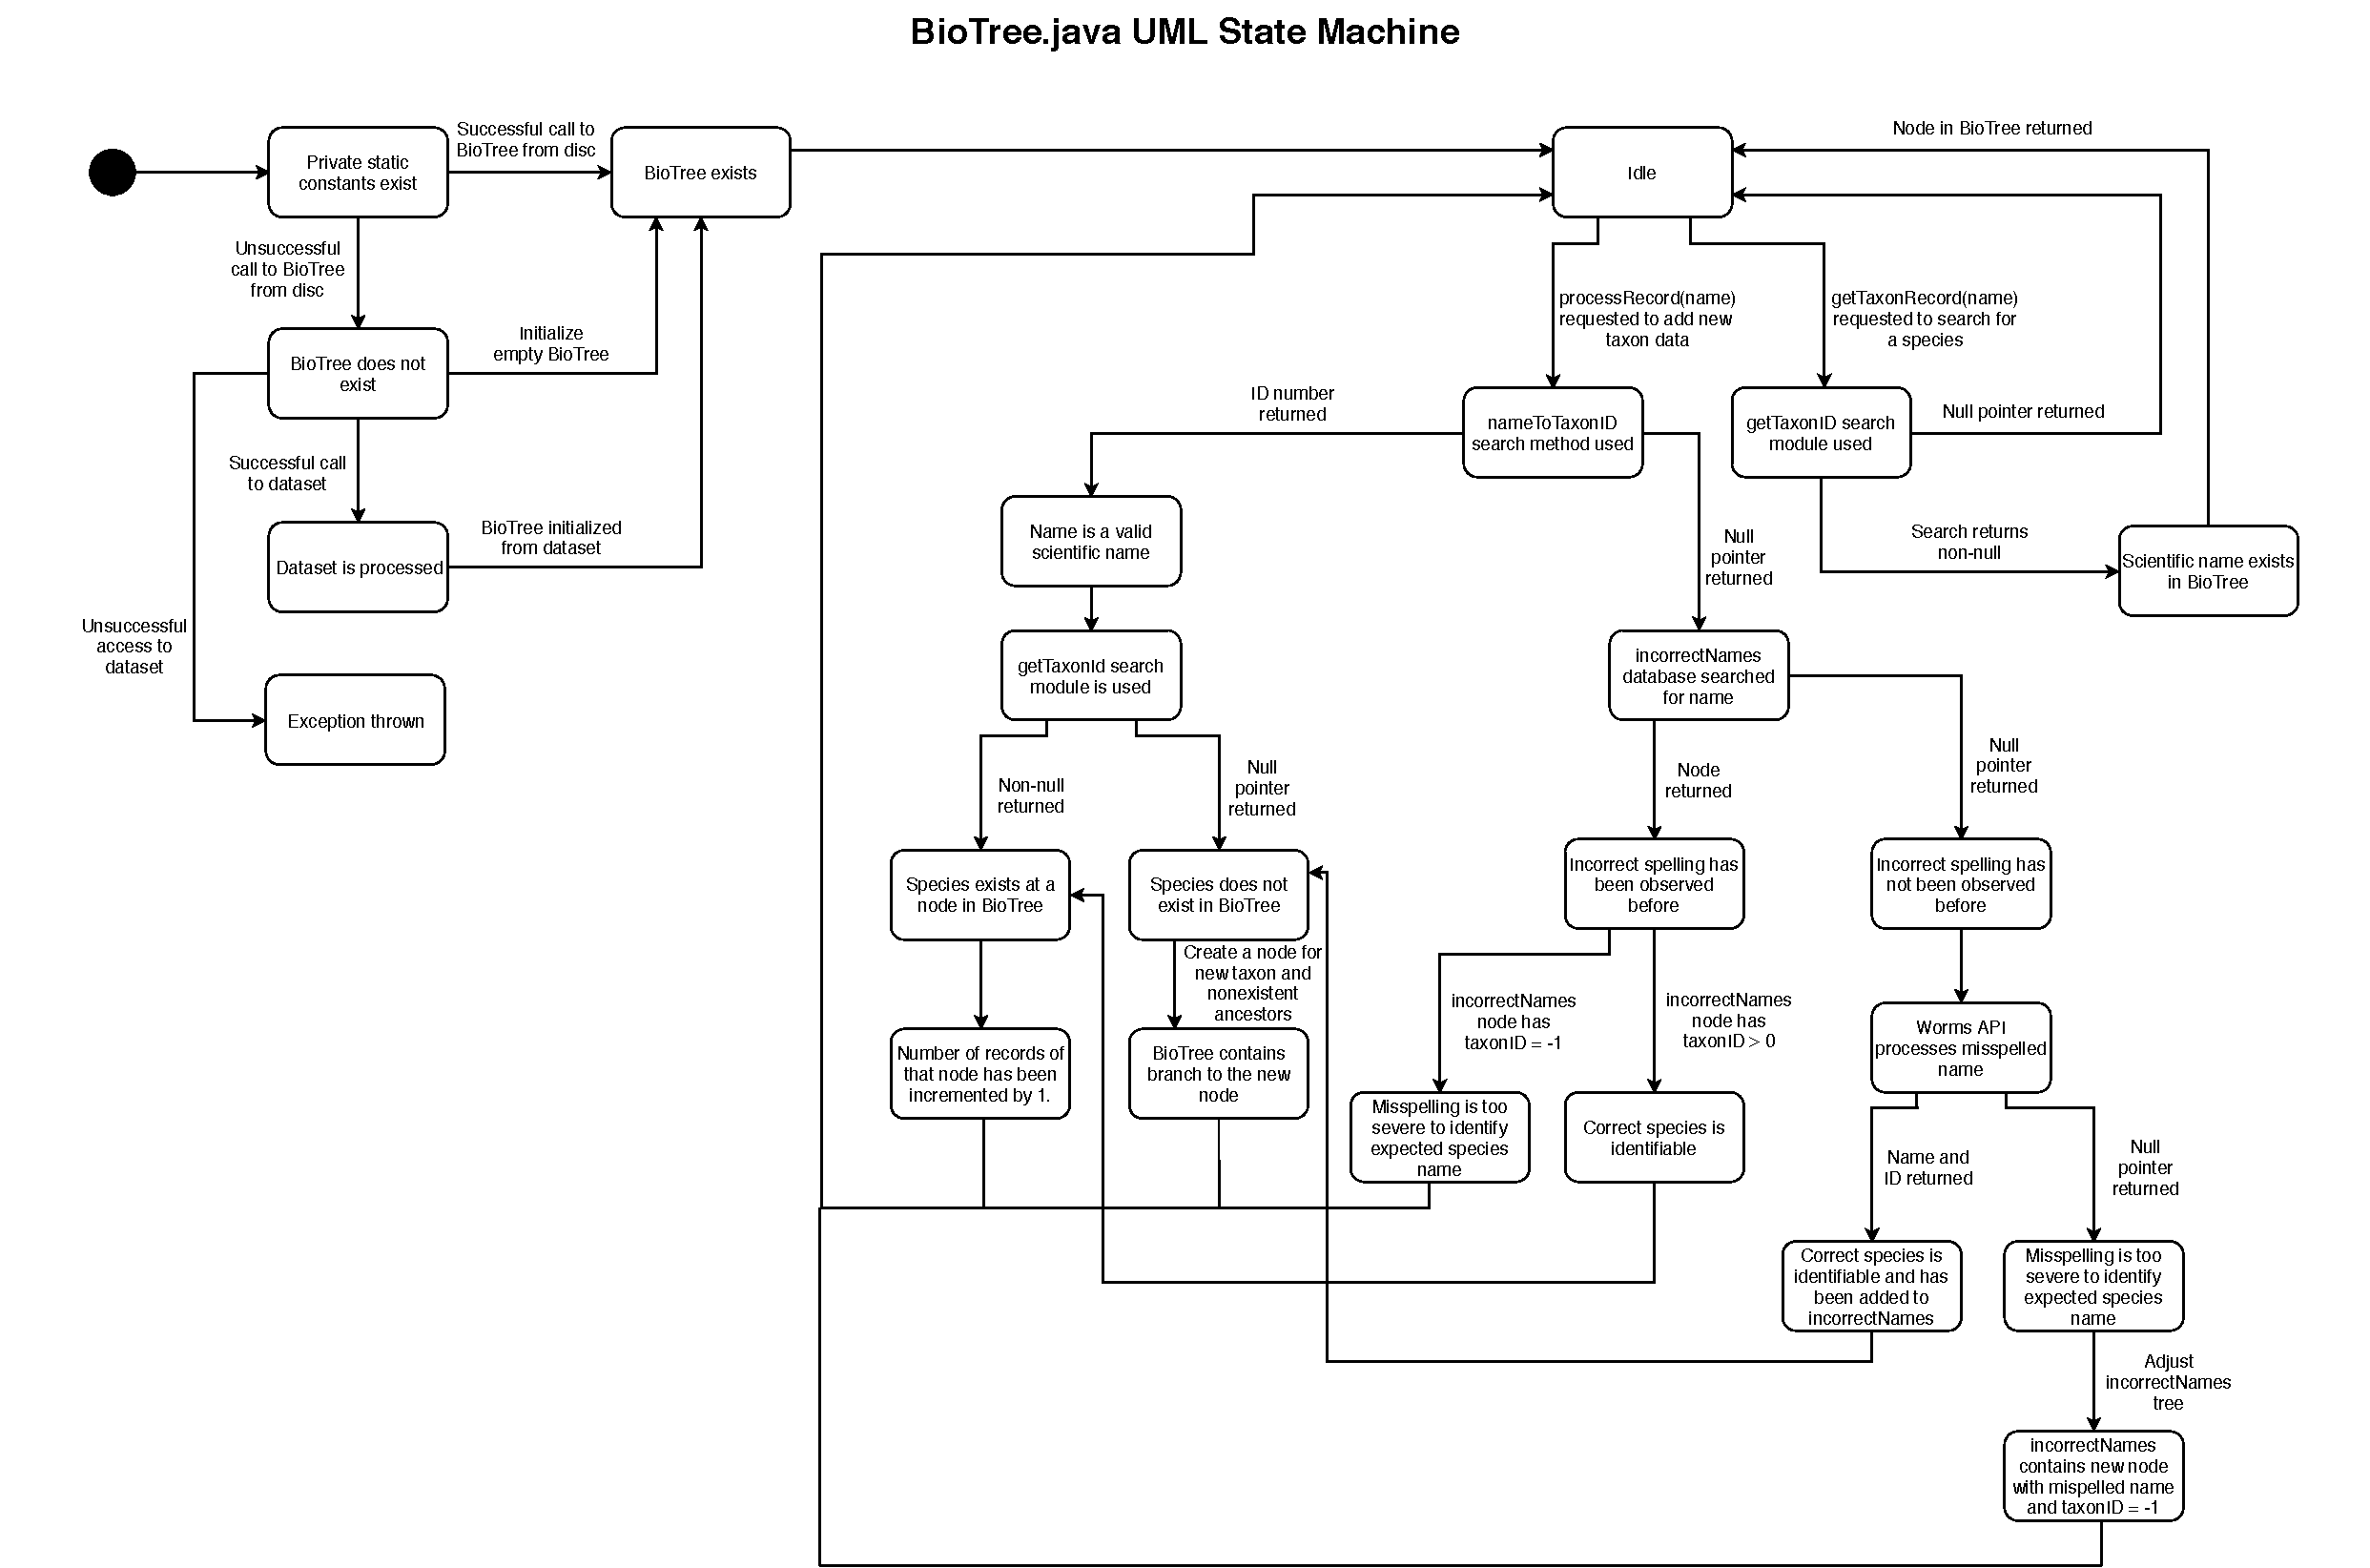
\includegraphics[width=18cm, trim={0 0 0 0}, clip]{BioTreeDotJava.pdf}

\caption{UML State machine diagram for \textit{/data/biotree/BioTree.java}, a class that builds a tree data structure from the scientific name hierarchies (called taxa) of fish. Uses a World Register of Marine Species (Worms) API to identify the correct spelling of species names for misspelled scientific names in the dataset. }
\label{fig:BioTreeUML}
\end{figure}


\section{Algorithmic Opportunities}
The \textit{TrawlExpert} was made possible by the use of vaious algorithms studied in \textit{SFWRENG 2C03: Algorithms} offered at McMaster University. These algorithms include \textit{Red-Black Tree} for searching and \textit{Merge Sort} for sorting objects. Additional algorithms outside of the course scope were implemented to optimize the program; they are described below. 

\subsection{Quick Select}
A modified form of the \textit{Quick Sort} algorithm that returns the $k^{th}$ largest element of an unsorted array. Similar to \textit{Quick Sort}, \textit{Quick Select} randomly chooses a partitioning element to sort the array such that all elements smaller than the partition are left of it, and larger elements are to the right. However, rather than recursively sorting both halves of the partitioned array, \textit{Quick Select} only sorts the half containing the $k^{th}$ index. The algorithm terminates once the partitioning element ends up at the $k^{th}$ index of the array, the value of this element is returned.

This algorithm is implemented in \textit{/sort/QuickSelect.java}. It is used during the construction of \textit{k-d tree}s which require the frequent division of an array into two equally sized halves. By finding the median element of an array, it is partially sorted into equally sized small and large halves. The \textit{Quick Select} class implements a \textit{median} method to simplify its usage in \textit{k-d tree} construction. 

% Mention optimization for Worms API

\subsection{kd Tree}
A k-dimensional (kd) binary search tree was used to provide a fast range searching structure for the records. Given that the current size of the USGS dataset is over 280,000 entries and likely to grow with additional studies, it was crucial to have a structure to support fast searches. However, since the data contains many dimensions (taxon id, latitude, longitude, date), a simple binary search tree is not useful for this task. Instead, a kd-tree was employed.

A kd-tree is like a binary search tree except that on each level $i$ of the tree, the comparison between nodes is made on the ($i\ \%\ d$)th axis of the data. For example, in a two-dimensional tree of ($x,y$) points, the first level of the tree would be compared on $x$, and the second level would be compared on $y$, the third level on $x$, and so on.

This structure gives a fast way of range searching for values in the tree, with a search complexity of $\mathcal{O}(dn^{1-\frac{1}{d}})$ where $n$ is the number of nodes in the tree and $d$ is the number of splitting dimensions of the tree. In the \textit{TrawlExpert}, we use a 4-d tree to split on taxon id, date, latitude and longitude. Range searches for specific species are very fast, often on the order of 5-10ms and sometimes as fast as 1ms.

In order to build the kd-tree in a balanced way, it's crucial to be able to find the median of the data, so that a balanced number of nodes are inserted on each left and right subtree within the tree. In order to support fast $kd$ tree building (which only needs to happen once when the dataset is first analyzed), the aforementioned \textit{QuickSelect} algorithm was used, which was able to allow building the whole kd-tree in about 0.6 seconds. The kd-tree class then contains methods for serializing the data of the kd-tree so that it can be reloaded quickly from the disc on subsequent launches of \textit{TrawlExpert}.

%
% Chris will write :) ============================ LOOK HERE CHRIS =================================
%

\subsection{Graphing}
Graph algorithms were used to support advanced searching features. Firstly, the biological classification of each organism forms a tree from which species in the same genus, for example, can be located. This was accomplished by creating a BioTree node, which stores the taxon id number of the classification, the scientific name of the entry, the number of records with that taxon id contained in the dataset and pointers to the parent and the children of the node. This structure directly mimics the method that scientists use to classify species according to their similarities (into family, genus, species) and allows for intelligent filtering and searching of the dataset. For example, with this structure it is possible to find all descendants of a certain biological classification.

Secondly, a graph algorithm was used to find connected components among search results. Nodes are connected together based on their distance to surrounding points \citep{tom10}. Depth-first search was used to determine connected components \citep{broder2000graph}.

\section{Software Design Principles}
\subsection{Robustness}
Robustness is a non-functional requirement prioritized during the \textit{TrawlExpert}'s development. Considering all 280,000+ records in the dataset were entered by humans, data entry errors were inevitable. The \textit{TrawlExpert} implementation had to ensure unexpected entries in the dataset were handled gracefully and could be recovered if possible. 

When building a BioTree from the dataset, the World Register of Marine Species (WORMS) database API was used to find the correct scientific name of slightly misspelled names. Unless a name was severely misspelled, the Worms API was able to salvage small data entry errors. This ensured records could be used when building the BioTree and protected the tool from raising exceptions from small input errors. While this introduces a dependance on an Internet connection to \textit{TrawlExpert}, it was assumed that the scientists working with \textit{TrawlExpert} would have access to an Internet connection, and the tradeoff is reasonable for the recovery of many errors in the dataset.

The use of drop-down boxes on the user interface helped limit invalid search criteria from being entered. From left to right, each box contains increasingly specific components of a scientific name for fish species. When any of the dropdown boxes were selected, all boxes to the left (representing more general components of that species name) were updated. This was to ensure the hierarchy formed by the more general components contained the newly adjusted value. Additionally, all boxes to the right were cleared. If a more general feature was adjusted, the resultant possible species no longer satisfies the hierarchy needed by values populating the right-most boxes. To prevent invalid scientific names from being used as search input, they had to be cleared. 

\subsection{Scalability}
The tool must be able to handle large amounts of data, all while being able to complete queries at a high speed. Currently, the tool uses a dataset of 200,000 lines of data, but it must be able to maintain its high performace for larger datasets. Using sorting algorithms such as \textit{Quick Select} to build a \textit{k-d tree}, the \textit{TrawlExpert} has been optimized to complete tree construction much faster.

Implementing \textit{Quick Select} rather than \textit{Merge Sort} drastically improved the \textit{TrawlExpert}'s performance. When using \textit{Merge Sort} during \textit{k-d tree} construction, an array must be fully sorted before retrieving the median element, taking $\mathcal{O}(n\lg n)$ time where $n$ is the size of the dataset. \textit{Quick Select} only partially sorts the array before reaching the median, taking $\mathcal{O}(n)$ time, and it reduced \textit{k-d tree} construction from 40.083 s using \textit{Merge Sort} to 0.56 s, representing a 72x improvement. 

\subsection{Generality}
A common theme among \textit{TrawlExpert} classes is the use of lambda functions characterized by Java interfaces which describe their syntax as well as their semantic meaning. Lambda functions provide the capacity for parameterized object comparison or parameterized value access. This maintains the generality, and therefore reusability, of each class by allowing for generic types in class definitions. Type(s) of the input(s) and the how input object(s) are used only become assigned when the function is used.

\subsubsection{General Compare}
The \textit{GeneralCompare} interface can be found at \textit{/sort/GeneralCompare.java}. This interface includes a \textit{compare} function that takes two generically typed inputs and produces an integer output. When \textit{GeneralCompare} is used in other classes, a compare function (the lambda function) is used to instantiate the expected input type and designate how the integer result must be calculated. This allows reuse of the interface among modules that perform comparisons of differently typed objects. Two records consisting of a fish species, date of observation, and geographic location can be compared based on lexicographic order of their names, date, or proximity to some location. \textit{GeneralCompare} enables the comparison of record objects based on any of these parameters. 

\subsubsection{Field}
The \textit{Field} interface can be found at \textit{/search/Field.java}. This interface includes a \textit{field} function that retrieves a key (a generic type) from a generically typed input object. Similar to \textit{GeneralCompare}'s \textit{compare} function, \textit{field} is a lambda function. The field interface is used to perform searches in a tree of records that have been sorted by variable attributes from each record. The lambda function specifies which attribute to access when searching through the tree.

\subsubsection{General Range}
The \textit{GeneralRange} interface can be found at \textit{/sort/GeneralRange.java}. This interface includes a \textit{isInBounds} function returns an integer to describe if a record is member to a subset of the search results. The input has a generic type, rather than \textit{Record} type, to satisfy reusability. The lambda function uses the range itself to perform conditional checks about whether the input object is below, within, or above the range. A return value of -1 indicates it is below, 0 indicates it is within, and 1 indicates it is above the range.

\section{Internal Review}
\subsection{Meeting Functional Requirements}
The first challenge in developing this tool was parsing the data. One requirement was to read and clean the data, then produce a data structure of Record objects. The software tool performed this task as planned, and even exceeded expectations by using a \textit{k-d tree} to store the Records in an easily accessible manner. Another requirement was to accomplish basic searching capabilities based on input criteria. This aspect was achieved through efficient sorting and searching algorithms, the results were verified using JUnit test cases of all searching and sorting algorithms.

\subsection{Meeting Non-Functional Requirements}
In terms of meeting non-functional requirements, the team met expectations. The use of the Worms API when parsing the dataset improved robustness and algorithmic choices such as \textit{Quick Select} and \textit{k-d tree}s improved performance. The final product achieved the requirement of being user-friendly since it is easily accessible via the Google Cloud server and prevents the user from entering invalid search criteria. 

Additional goals included using less than 1 GB of RAM, this was achieved since the \textit{TrawlExpert} used approximately 0.5 GB of RAM. An additional goal was to perform queries in less than 1 second, this was achieved. A positive team dynamic throughout the development process ensured collaboration and help were always offered, this was a large contributing factor to the success of the final product. 

\subsection{Changes During Development}
There were some algorithmic changes that were realized during development. Two key algorithmic changes were the change from \textit{Merge Sort} to using \textit{Quick Select}, and changing cluster groups of Connected Components. As discussed in Algorithmic Opportunities, the use of \textit{Quick Select} dramatically improved performance. 

Another algorithmic change involved the client code for Connected Components when determining fish clusters. Initially, every node was visited multiple times to determine whether other nodes were within a given radius. The running time was unacceptable using this approach, and as a result, the algorithm was changed such that visited nodes were not revisited. This decreased running time significantly and was considered acceptable by the team. 

\subsection{Future Changes}
While \textit{TrawlExpert} met all of its original goals for this stage of its development, there are several points for improvement and future development of the platform as an all-in-one research tool for watershed research.

\subsubsection{Improvements on Development Process}
Most of the changes that would benefit the \textit{TrawlExpert} involve its development requirements. The original goals for this section were quite extensive, however one aspect that was overlooked was file organization. Although GitLab was used for version control, confusion still occurred over which packages certain classes belonged to. For example, there were instances in the project where a search class would be located in the graph package. Adding a requirement for file organization would make the project more easily accessible in the development process and would also yield more efficient workflow because less time would be dedicated to searching for a desired class. 

\subsubsection{Future Functionality}
Functionally, there are many future goals in the development of \textit{TrawlExpert}. This phase of the development process was aimed at providing scientists with an effective tool to search and filter data relevant to their research, as well as some basic statistical tools. However, this only represents the first stage in a larger scientific research pipeline. Often, more advanced tools such as stratified statistical analysis is needed to properly take into account the many variables in trawl survey expeditions (FIXME: ref). The future work includes building these tools into \textit{TrawlExpert} in order to create an all-in-one research platform for trawl surveys.

\clearpage
\bibliographystyle{apa}
\bibliography{bib}


\end{document}